\subsection{Direct Transfer of the Submitted Hackathon System}
\label{sec:historical-transfer}

Before the confirmatory continuous study, the unchanged submitted ZIP
and an earlier physical estimator were executed on the same \HistoryWindows{}
windows: \HistoryEvents{} event realizations and \HistoryNormals{} normal windows.
Figure~\ref{fig:historical-transfer} preserves their actual family
confusions. The submitted ExtraTrees pipeline detected \HistoryETDetected{}
of the \HistoryEvents{} events, assigned the right family to
\HistoryETFamily{}, and the right family and exact source to
\HistoryETJoint{}. The earlier physical estimator obtained
\HistoryPhysicalJoint{}/\HistoryEvents{} for all
three quantities. Neither alarmed in the 28 normal windows. The source
result was checked against the submission's output CSVs, not inferred
from the family matrix.

\begin{figure*}[t]\centering
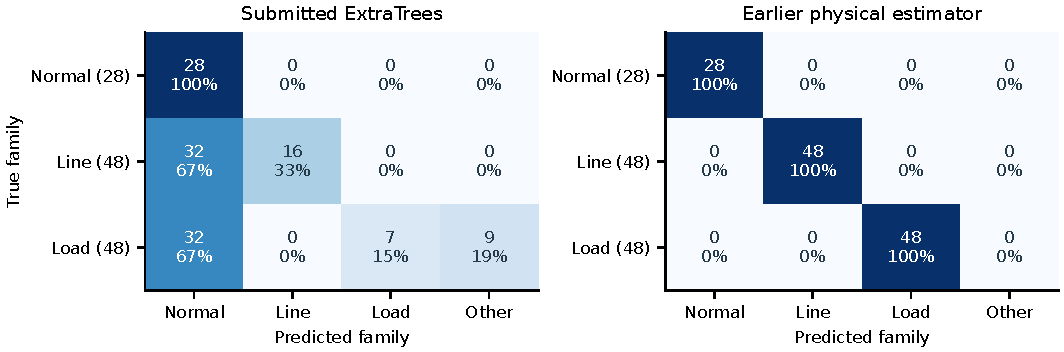
\includegraphics[width=.96\textwidth]{figures/generated/historical_transfer_confusion.pdf}
\caption{Historical development transfer on shared observation windows.
Cells show counts and row percentages. All out-of-scope predictions are
retained as ``Other''; the submitted system's nine such predictions were
the unknown-event label. This is a family matrix, not a localization
matrix. The physical comparator is an earlier estimator, not the final
continuous bank. The 96 event realizations reuse 36 physical event
trajectories; the normal windows come from six physical trajectories.}
\label{fig:historical-transfer}\end{figure*}

This comparison exposes a transfer failure of the delivered system on
the later simulator's load/line catalog. It does not show an official
hackathon-score improvement. The submitted model retains its broader
training domain and 30-s window rule, whereas the physical estimator
knows the simulator and its 12 candidate origins. These were development
cases, and the comparison permits both methods the same window endpoint.
The next study therefore uses separately trained causal ExtraTrees
comparators, successive events and a new frozen cohort. Its results must
be read as a second experiment, not as more independent repetitions of
the perfect development score.
